\documentclass[border=4pt,12pt]{standalone}
% House style for redrawn exam diagrams (diagram-v4: 0.4pt lines, filled -latex arrows, fine dashes; stipple and hatching drawn as real dots/lines (no PDF/SVG patterns, so they render in every browser and at any scale); transparent background). Every figure \input's this.
\usepackage{amsmath,amssymb}
\usepackage{txfonts}
\usepackage{pdfrender,xcolor}
% \halo{text}: label on shading. The shading stops just around each letter's outline (a thin knock-out that follows the
% glyphs, like the papers' typesetting), never a box. Owner: "I don't want a box around the text".
\newcommand{\halo}[1]{\leavevmode\rlap{\pdfrender{TextRenderingMode=2,LineWidth=2.2pt,LineJoinStyle=1,StrokeColor=white,FillColor=white}#1}#1}
\usepackage{tikz,pgfplots}
\pgfplotsset{compat=1.18}
\usetikzlibrary{arrows.meta,calc,angles,quotes,patterns,patterns.meta,intersections,positioning,decorations.markings,shapes.geometric}
% Stipple and hatching are drawn as actual dots / lines clipped to the region (path picture), NOT as pattern fills:
% SVG <pattern> fills vanish or blur when browsers scale the image, so the owner could not see the shading.
% Each dot is a 0.72pt square (keeps SVGs small; reads as a dot at print size). Dots sit on one global staggered grid, so neighbouring regions line up.
\makeatletter
\newdimen\ex@x \newdimen\ex@y \newdimen\ex@xa \newdimen\ex@ya \newdimen\ex@xb \newdimen\ex@yb \newcount\ex@row
\def\exam@stipplecolor{black!75}\def\exam@dotr{0.42pt}\def\exam@dotgap{2.5}
\def\ex@rowdots{\ifdim\ex@x<\ex@xb \pgfpathrectangle{\pgfqpoint{\dimexpr\ex@x-0.36pt\relax}{\dimexpr\ex@y-0.36pt\relax}}{\pgfqpoint{0.72pt}{0.72pt}}\advance\ex@x by \exam@dotgap pt\relax\expandafter\ex@rowdots\fi}
\def\exam@stipple{%
  \pgftransformreset% dots are sized in real points even inside scaled pictures
  \pgfpointanchor{path picture bounding box}{south west}\ex@xa=\pgf@x \ex@ya=\pgf@y
  \pgfpointanchor{path picture bounding box}{north east}\ex@xb=\pgf@x \ex@yb=\pgf@y
  \pgfsetfillcolor{\exam@stipplecolor}\pgfmathsetmacro\ex@h{\exam@dotgap/2}%
  \pgfmathtruncatemacro\ex@r{floor(\ex@ya/\ex@h)-1}\ex@row=\ex@r\relax
  \ex@y=\ex@r\dimexpr\ex@h pt\relax
  \loop\ifdim\ex@y<\ex@yb
    \pgfmathtruncatemacro\ex@c{floor(\ex@xa/\exam@dotgap)-1}\ex@x=\ex@c\dimexpr\exam@dotgap pt\relax
    \ifodd\ex@row \advance\ex@x by \ex@h pt\fi
    \ex@rowdots
    \advance\ex@y by \ex@h pt \advance\ex@row by 1
    \ifnum\numexpr\ex@row-(\ex@row/4)*4\relax=0 \pgfusepath{fill}\fi% flush every 4 rows: bounded TeX memory, few clip copies in the SVG
  \repeat\pgfusepath{fill}}
\newdimen\ex@d
\def\exam@hatch#1{% #1 = 1 for /, -1 for \ ; lines 45 degrees, 3pt apart
  \pgftransformreset
  \pgfpointanchor{path picture bounding box}{south west}\ex@xa=\pgf@x \ex@ya=\pgf@y
  \pgfpointanchor{path picture bounding box}{north east}\ex@xb=\pgf@x \ex@yb=\pgf@y
  \ex@d=\dimexpr\ex@yb-\ex@ya\relax \ex@x=\dimexpr\ex@xa-\ex@d\relax
  \loop\ifdim\ex@x<\ex@xb
    \ifnum#1>0 \pgfpathmoveto{\pgfqpoint{\ex@x}{\ex@ya}}\pgfpathlineto{\pgfqpoint{\dimexpr\ex@x+\ex@d\relax}{\ex@yb}}%
    \else \pgfpathmoveto{\pgfqpoint{\ex@x}{\ex@yb}}\pgfpathlineto{\pgfqpoint{\dimexpr\ex@x+\ex@d\relax}{\ex@ya}}\fi
    \advance\ex@x by 4.24pt
  \repeat
  \pgfsetlinewidth{0.4pt}\pgfsetstrokecolor{black}\pgfusepath{stroke}}
\def\examstipple{\exam@stipple}\def\examhatch{\exam@hatch}\def\examsetstipplecolor#1{\def\exam@stipplecolor{#1}}\def\examsetdotgap#1{\def\exam@dotgap{#1}}
\makeatother
% (legacy pattern kept for old files)
% staggered stipple like the NESA papers' dotted shading
\pgfdeclarepatternformonly{exam stipple}{\pgfpointorigin}{\pgfqpoint{2.2pt}{2.2pt}}{\pgfqpoint{2.2pt}{2.2pt}}{%
  \pgfpathcircle{\pgfqpoint{0.55pt}{0.55pt}}{0.42pt}\pgfpathcircle{\pgfqpoint{1.65pt}{1.65pt}}{0.42pt}\pgfusepath{fill}}
\tikzset{
  every picture/.style={line width=0.6pt, >={Latex[length=2mm,width=1.3mm]}},
  curve/.style={line width=0.6pt},
  open arrow/.style={-{Latex[length=2mm,width=1.3mm]}},  % owner: filled -latex heads everywhere, no open chevrons
  aux/.style={dash pattern=on 2pt off 1.5pt, line width=0.6pt},
  shade/.code={\def\exA{#1}\def\exB{none}\ifx\exA\exB\else\pgfkeysalso{fill=black!18}\fi},
  shade/.default=on,
  shade dots/.style={fill=none, path picture={\examstipple}},
  stipple color/.code={\examsetstipplecolor{#1}},
  stipple gap/.code={\examsetdotgap{#1}},
  shade dense dots/.style={fill=none, stipple gap=1.6, path picture={\examstipple}},
  shade hatch/.style={fill=none, path picture={\examhatch{1}}},
  shade hatch reverse/.style={fill=none, path picture={\examhatch{-1}}},
  shade solid/.style={fill=black},
  pt/.style={circle, fill, inner sep=1.1pt},
  open pt/.style={circle, draw, fill=white, inner sep=1.1pt},
}
\pgfplotsset{
  exam axes/.style={axis lines=middle, axis line style={->}, xlabel={$x$}, ylabel={$y$},
    xlabel style={anchor=west}, ylabel style={anchor=south}, tick label style={font=\small},
    every axis plot/.append style={line width=0.6pt, black}, samples=200, clip=false,
    enlargelimits=false, axis on top},
}

\begin{document}
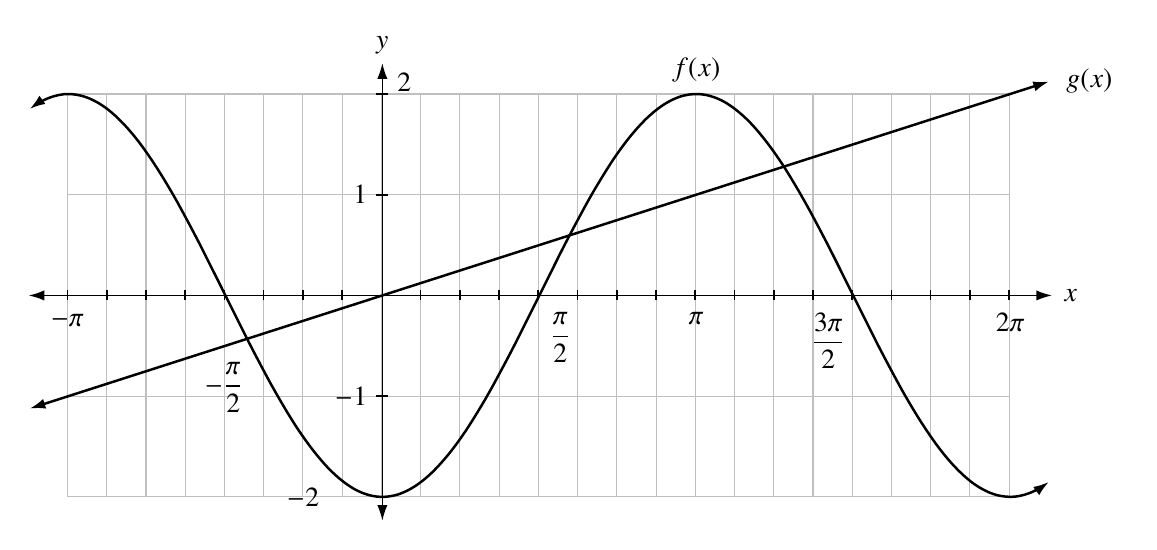
\begin{tikzpicture}[x=0.0127cm, y=-0.0127cm]
\draw[black!25, line width=0.4pt] (57.0,75.0) -- (57.0,478.0);
\draw[black!25, line width=0.4pt] (96.2,75.0) -- (96.2,478.0);
\draw[black!25, line width=0.4pt] (135.5,75.0) -- (135.5,478.0);
\draw[black!25, line width=0.4pt] (174.8,75.0) -- (174.8,478.0);
\draw[black!25, line width=0.4pt] (214.0,75.0) -- (214.0,478.0);
\draw[black!25, line width=0.4pt] (253.2,75.0) -- (253.2,478.0);
\draw[black!25, line width=0.4pt] (292.5,75.0) -- (292.5,478.0);
\draw[black!25, line width=0.4pt] (331.8,75.0) -- (331.8,478.0);
\draw[black!25, line width=0.4pt] (371.0,75.0) -- (371.0,478.0);
\draw[black!25, line width=0.4pt] (410.2,75.0) -- (410.2,478.0);
\draw[black!25, line width=0.4pt] (449.5,75.0) -- (449.5,478.0);
\draw[black!25, line width=0.4pt] (488.8,75.0) -- (488.8,478.0);
\draw[black!25, line width=0.4pt] (528.0,75.0) -- (528.0,478.0);
\draw[black!25, line width=0.4pt] (567.2,75.0) -- (567.2,478.0);
\draw[black!25, line width=0.4pt] (606.5,75.0) -- (606.5,478.0);
\draw[black!25, line width=0.4pt] (645.8,75.0) -- (645.8,478.0);
\draw[black!25, line width=0.4pt] (685.0,75.0) -- (685.0,478.0);
\draw[black!25, line width=0.4pt] (724.2,75.0) -- (724.2,478.0);
\draw[black!25, line width=0.4pt] (763.5,75.0) -- (763.5,478.0);
\draw[black!25, line width=0.4pt] (802.8,75.0) -- (802.8,478.0);
\draw[black!25, line width=0.4pt] (842.0,75.0) -- (842.0,478.0);
\draw[black!25, line width=0.4pt] (881.2,75.0) -- (881.2,478.0);
\draw[black!25, line width=0.4pt] (920.5,75.0) -- (920.5,478.0);
\draw[black!25, line width=0.4pt] (959.8,75.0) -- (959.8,478.0);
\draw[black!25, line width=0.4pt] (999.0,75.0) -- (999.0,478.0);
\draw[black!25, line width=0.4pt] (57,478.0) -- (999.0,478.0);
\draw[black!25, line width=0.4pt] (57,377.25) -- (999.0,377.25);
\draw[black!25, line width=0.4pt] (57,175.75) -- (999.0,175.75);
\draw[black!25, line width=0.4pt] (57,75.0) -- (999.0,75.0);
\draw[<->] (18,276.5) -- (1042,276.5);
\draw[<->] (372,502) -- (372,44);
\draw (57.0,271.5) -- (57.0,281.5);
\draw (96.2,271.5) -- (96.2,281.5);
\draw (135.5,271.5) -- (135.5,281.5);
\draw (174.8,271.5) -- (174.8,281.5);
\draw (214.0,271.5) -- (214.0,281.5);
\draw (253.2,271.5) -- (253.2,281.5);
\draw (292.5,271.5) -- (292.5,281.5);
\draw (331.8,271.5) -- (331.8,281.5);
\draw (410.2,271.5) -- (410.2,281.5);
\draw (449.5,271.5) -- (449.5,281.5);
\draw (488.8,271.5) -- (488.8,281.5);
\draw (528.0,271.5) -- (528.0,281.5);
\draw (567.2,271.5) -- (567.2,281.5);
\draw (606.5,271.5) -- (606.5,281.5);
\draw (645.8,271.5) -- (645.8,281.5);
\draw (685.0,271.5) -- (685.0,281.5);
\draw (724.2,271.5) -- (724.2,281.5);
\draw (763.5,271.5) -- (763.5,281.5);
\draw (802.8,271.5) -- (802.8,281.5);
\draw (842.0,271.5) -- (842.0,281.5);
\draw (881.2,271.5) -- (881.2,281.5);
\draw (920.5,271.5) -- (920.5,281.5);
\draw (959.8,271.5) -- (959.8,281.5);
\draw (999.0,271.5) -- (999.0,281.5);
\draw (366,478.0) -- (378,478.0);
\draw (366,377.25) -- (378,377.25);
\draw (366,175.75) -- (378,175.75);
\draw (366,75.0) -- (378,75.0);
\draw[line width=0.9pt,<->] plot[smooth] coordinates {(19.1,90.1) (27.6,84.2) (36.2,79.8) (44.8,76.8) (53.3,75.2) (61.9,75.2) (70.5,76.6) (79.1,79.5) (87.6,83.8) (96.2,89.5) (104.8,96.7) (113.3,105.1) (121.9,114.8) (130.5,125.7) (139.0,137.7) (147.6,150.7) (156.2,164.7) (164.8,179.4) (173.3,194.9) (181.9,211.0) (190.5,227.5) (199.0,244.5) (207.6,261.6) (216.2,278.9) (224.8,296.1) (233.3,313.2) (241.9,330.1) (250.5,346.5) (259.0,362.4) (267.6,377.7) (276.2,392.3) (284.7,406.0) (293.3,418.7) (301.9,430.4) (310.5,441.0) (319.0,450.4) (327.6,458.4) (336.2,465.2) (344.7,470.6) (353.3,474.5) (361.9,477.0) (370.4,478.0) (379.0,477.5) (387.6,475.6) (396.2,472.1) (404.7,467.3) (413.3,461.0) (421.9,453.4) (430.4,444.5) (439.0,434.4) (447.6,423.1) (456.2,410.7) (464.7,397.3) (473.3,383.1) (481.9,368.0) (490.4,352.3) (499.0,336.1) (507.6,319.4) (516.1,302.3) (524.7,285.1) (533.3,267.9) (541.9,250.7) (550.4,233.6) (559.0,216.9) (567.6,200.7) (576.1,185.0) (584.7,169.9) (593.3,155.7) (601.8,142.3) (610.4,129.9) (619.0,118.6) (627.6,108.5) (636.1,99.6) (644.7,92.0) (653.3,85.7) (661.8,80.9) (670.4,77.4) (679.0,75.5) (687.6,75.0) (696.1,76.0) (704.7,78.5) (713.3,82.4) (721.8,87.8) (730.4,94.6) (739.0,102.6) (747.5,112.0) (756.1,122.6) (764.7,134.3) (773.3,147.0) (781.8,160.7) (790.4,175.3) (799.0,190.6) (807.5,206.5) (816.1,222.9) (824.7,239.8) (833.2,256.9) (841.8,274.1) (850.4,291.4) (859.0,308.5) (867.5,325.5) (876.1,342.0) (884.7,358.1) (893.2,373.6) (901.8,388.3) (910.4,402.3) (919.0,415.3) (927.5,427.3) (936.1,438.2) (944.7,447.9) (953.2,456.3) (961.8,463.5) (970.4,469.2) (978.9,473.5) (987.5,476.4) (996.1,477.8) (1004.7,477.8) (1013.2,476.2) (1021.8,473.2) (1030.4,468.8) (1038.9,462.9)};
\draw[line width=0.9pt,<->] (19.1,389.7) -- (1038.9,62.5);
\node[anchor=north, inner sep=3pt] at (57,284.5) {$-\pi$};
\node[anchor=north, inner sep=0pt] at (214,342.5) {$-\dfrac{\pi}{2}$};
\node[anchor=north, inner sep=3pt] at (550,284.5) {$\dfrac{\pi}{2}$};
\node[anchor=north, inner sep=3pt] at (686.0,284.5) {$\pi$};
\node[anchor=north, inner sep=3pt] at (818,284.5) {$\dfrac{3\pi}{2}$};
\node[anchor=north, inner sep=3pt] at (1000.0,284.5) {$2\pi$};
\node[anchor=west, inner sep=3pt] at (378,63.0) {$2$};
\node[anchor=east, inner sep=3pt] at (366,175.75) {$1$};
\node[anchor=east, inner sep=3pt] at (366,377.25) {$-1$};
\node[anchor=east, inner sep=3pt] at (318,478.0) {$-2$};
\node[anchor=west, inner sep=3pt] at (1044,276.5) {$x$};
\node[anchor=south, inner sep=3pt] at (372,44) {$y$};
\node[anchor=south, inner sep=4pt] at (686.0,75.0) {$f(x)$};
\node[anchor=west, inner sep=6pt] at (1038.9,62.5) {$g(x)$};
\end{tikzpicture}
\end{document}
